\chapter{内存管理}



\section{虚拟地址转换}


\begin{figure}[htbp]
\centering 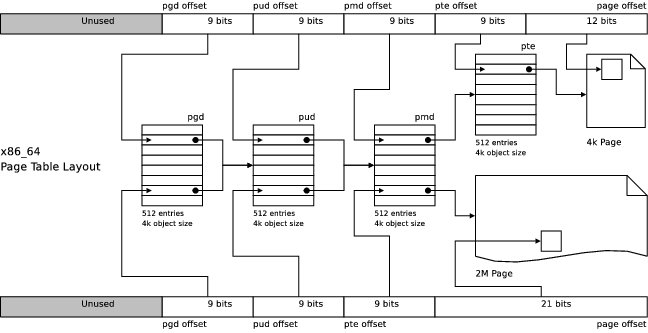
\includegraphics[width=1\textwidth]{va-to-pa.png}
\caption{虚拟地址转换\cite{linuxmm}}
\end{figure}

\section{页表结构}

\begin{figure}[htbp]
\centering 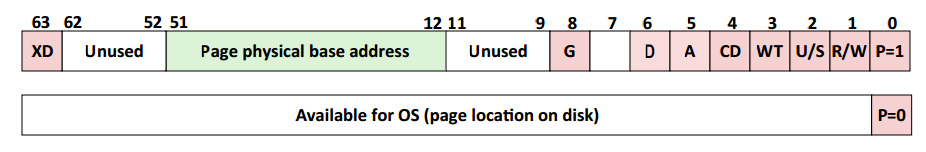
\includegraphics[width=1\textwidth]{pte.png}
\caption{Core i7 Level 4 Page Table	Entries}
\end{figure}

\begin{itemize}
\item \textbf{P:} Child page is present in memory (1)or not(0)	
\item \textbf{R/W:} Read-only or read-write access permission for child page	
\item \textbf{U/S:} User or	supervisor mode	access	
\item \textbf{WT:} Write-through or	write-back cache policy for this page	
\item \textbf{CD:} Cache disabled (1) or	enabled (0)	
\item \textbf{A:} Reference bit (set by MMU on reads and	writes, cleared	by sohware)		
\item \textbf{D:} Dirty bit (set	by MMU on writes, cleared by sohware)	
\item \textbf{G:} Global	page (don’t	evict from TLB on task switch)	
\item \textbf{Page physical base address:} 40 most significant bits of physical page address (forces pages to be	4KB	aligned)	
\end{itemize}
